\chapter{Conclusiones}

\section{Conclusiones Generales}
    
    La técnica de Divide y Vencerás se torno difícil para nosotros a la hora de aplicarla al algoritmo propuesto para esta práctica. Repasamos los temas y vimos que nuestro punto bajo era la aplicación de funciones que no habíamos trabajado en el lenguaje Python. 

    Concluyendo que reforzar el tema de Divide y Vencerás no solamente ayuda al análisis de algoritmos sino que es un aprendizaje que se puede llevar a todos lados con su filosofía. 

\newpage
\section{Isaac Sánchez - Conclusiones}
    Esta práctica me resultó confusa, ya que la codificación del algoritmo para cambiar de posición las matrices de la imagen jamás lo había visto. Graias al aprendizaje de divide y vencerás pude entrar en detalle para poder lograrlo. Presentamos problemáticas de tiempo para concretar los problemas anexos. De ahí en fuera, fue una práctica que reforzó mis conocimientos.
    \begin{figure}[htp!]
            \centering
            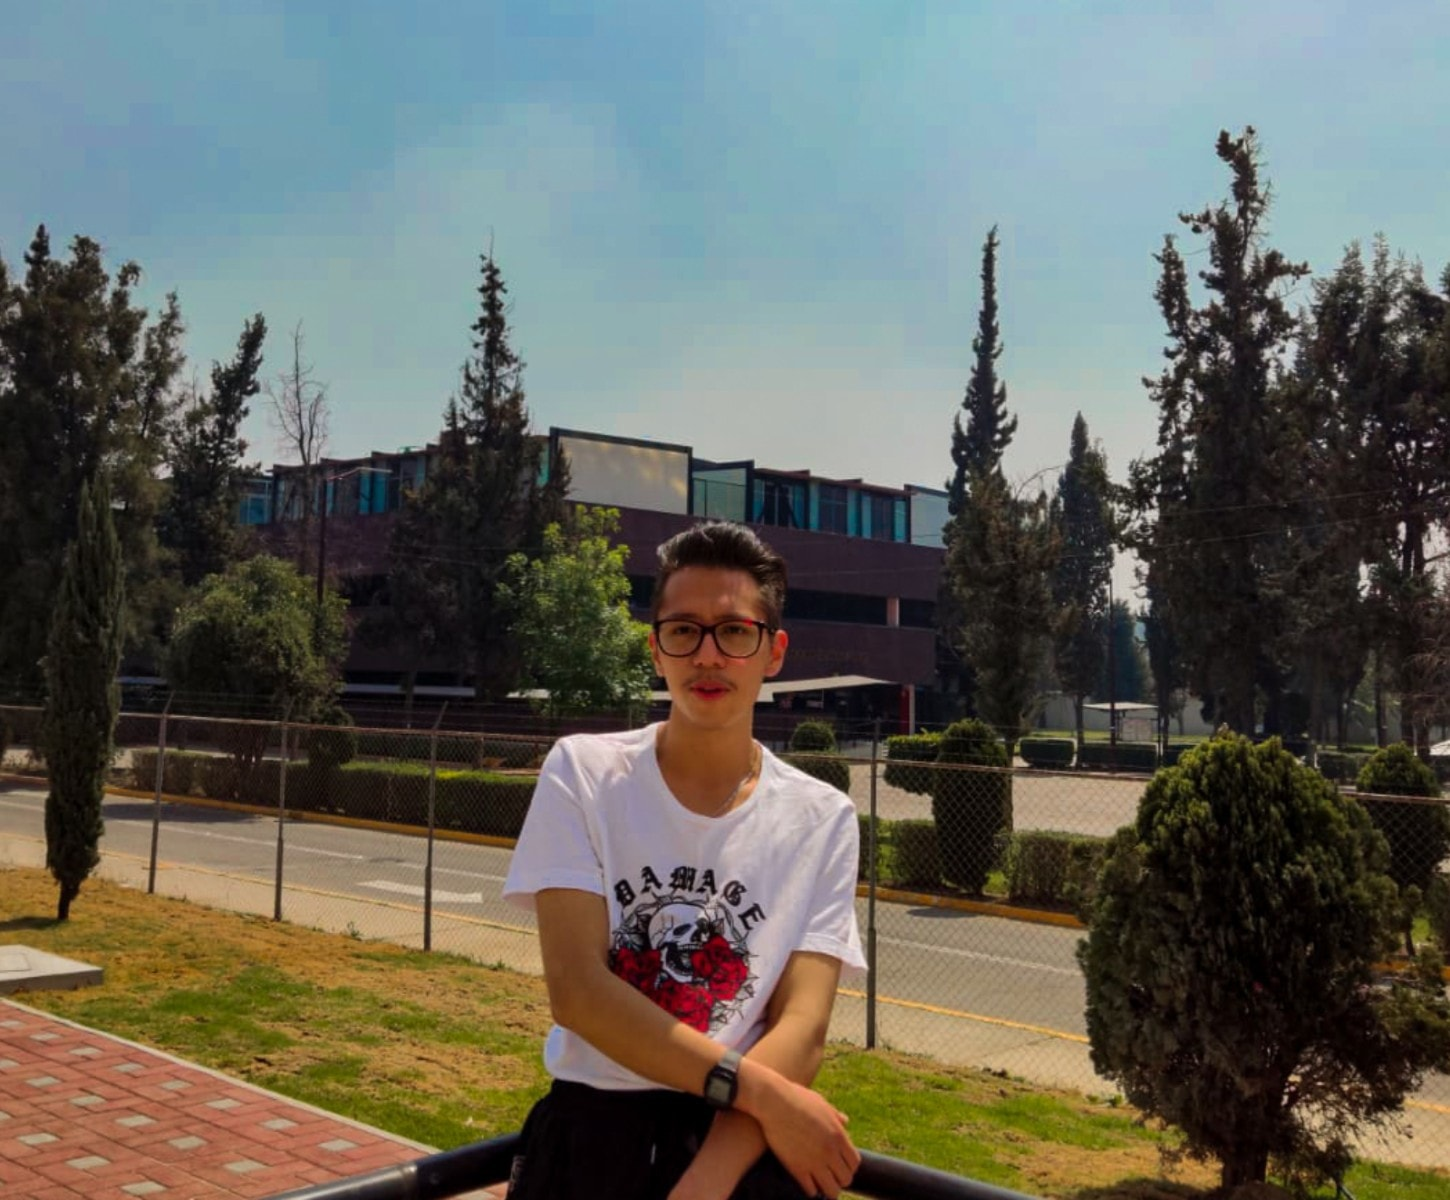
\includegraphics[width=1 \textwidth]{Images/Fotos_Alumnos/274612600_2528992867236334_6677874837890685705_n.jpg}  
            \caption{Isaac Sánchez}
            \label{fig:my_label1}
        \end{figure}
    


\newpage
\section{Axel Trevino - Conclusiones}
    Esta práctica es un buen ejemplo de los resultados de la recursividad adicionada al divide y vencerás, ya que cuando se piensa de manera normal, para rotar la imagen se tendrían que hacer dos cosas: cambiar los cuadrantes y rotarlos; pero al pensar que los cuatro cuadrantes igualmente son imágenes, sólo hay que aplicar el algoritmo ad infinitum y ya, todo se resuelve con el mismo proceso
    \begin{figure}[htp!]
            \centering
            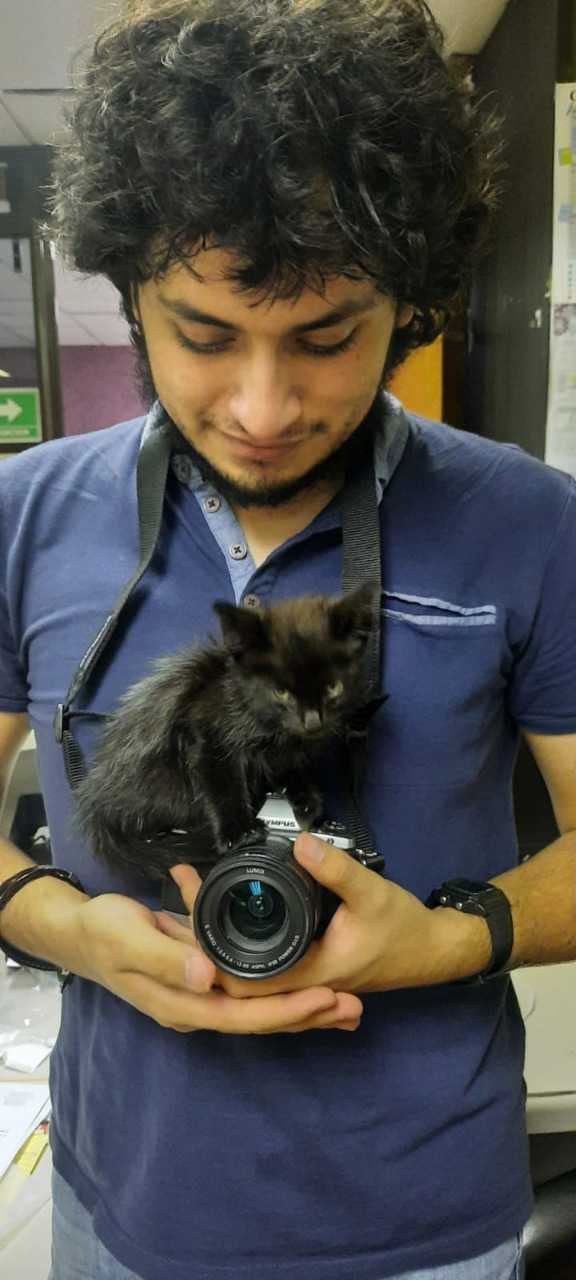
\includegraphics[width=0.4 \textwidth]{Images/Fotos_Alumnos/axel.jpg}  
            \caption{Axel Treviño}
            \label{fig:my_label2}
        \end{figure}
